\documentclass[12pt]{scrartcl}

\usepackage{float}

\usepackage[utf8]{inputenc}

\usepackage[T1]{fontenc}

\usepackage{lmodern}

\usepackage[ngerman]{babel}

\usepackage{amsmath}

\usepackage{graphicx}


 

\title{Versuch WO3\\ Beugung und Interferenz von Lichtwellen}

\author{Frederik Strothmann, Henrik Jürgens}

\date{\today}


\begin{document}


 %deckblatt erstellen

\maketitle
\tableofcontents
\newpage

%einleitung zu dem experiment

\section{Einleitung}

In der Versuchsreihe WO3 soll die Beugung (Diffraktion) von kohärenten Lichtwellen (Laserlicht) an verschiedenen Öffnungen untersucht werden.
Die Erscheinungen von Beugung und Interferenz sind grundlegend für die Wirkungsweise wichtiger optischer Instrumente. So bestimmt z.B. die Beugung an in der Regel kreisförmigen Öffnungen (z.B. Linsenfassungen) das räumliche Auflösungsvermögen aller optischer Instrumente vom Mikroskop über das menschliche Auge bis hin zu den großen Radioteleskopen. Wir werden zunächst die Intensitätsverteilung des Beugungsmusters eines Einzelspaltes ausmessen und unsere Messungen mit den entsprechenden Rechnungen, die auf dem Huygensschen Prinzip beruhen, vergleichen. Das gleiche werden wir dann anschließend mit den Beugungsbildern einer Lochblende, eines Doppelspaltes und eines Strichgitters durchführen.
%versuchsaufbau mit skizze

\section{Versuchsaufbau}

\section{Versuch WO3.1: Beugungsmuster eines Einfachspaltes}
\subsection{Versuchsdurchführung}

\subsubsection{Praktische Durchführung}
Wir bauen den in Abbildung 
%\ref{} Abbilung 17 aus der versuchsbeschreibung oder besser eine eigene zeichnung
skizzierten Versuchsaufbau mit Elementen der mikrooptischen Bank auf. Als Quelle für kohärente und ebene Wellen verwenden wir einen Neon-Helium-Gaslaser. Die Wellenlänge des Lichtes beträgt $\lambda$ = 0,6328 $\mu$m.
Wir messen die Intensitätsverteilung des Beugungsmusters in der Ebene des "Schirms" mit einem Intensitätsmessggerät aus. Wir tragen dann $\frac{I_\theta}{I_0}$ graphisch auf und vergleichen die Messwerte mit der theoretischen Verteilung. Aus der Lage der ersten Minima bestimmen wir die Wellenlänge $\lambda$.
\subsubsection{Theoretische Durchführung}
Den Winkel $\theta$ berechnen wir im folgenden \textbf{immer} mit der Formel:
\begin{align}
\theta = tan^{-1}(\frac{x}{L})
\end{align}
wobei x der Abstand zum Hauptmaximum und L der Abstand des Gitters zum Intensitätsmessgerät ist.\\
Der Fehler berechnet sich nach folgender Formel:
\begin{align}
\sigma_\theta = \sqrt{
\left(\frac{1}{L\left(1+\left(\frac{x}{L}\right)^2\right)}\sigma_x\right)^2+
\left(\frac{x}{L^2\left(1+\left(\frac{x}{L}\right)^2\right)}\sigma_L\right)^2}
\end{align}

Für die Intensitätsverteilung $I_\theta$ Abhängig vom Winkel $\theta$ erwarten wir folgenden Zusammenhang:
\begin{align}
I_\theta = I_0 \left(\frac{\sin \left(\frac{\pi b \sin{\theta}}{\lambda}\right)}{\frac{\pi b \sin{\theta}}{\lambda}}\right)^2
\end{align}
$I_0$ ist die Intensität bei einer Auslekung von 0$^{\circ}$, $b$ die Breite des Spaltes und $\lambda$ die Wellenlänge des Lasers.

Die Wellenlänge $\lambda$ kann aus der Lage des ersten Minimums bestimmt werden
\begin{align}
\lambda = \sin(\theta) b
\label{eqn:lambda_a_1}
\end{align}
$b$ ist dabei die Breite des Spaltes.\\
Der Fehler für die Wellenlänge ist:
\begin{align}
\sigma_\lambda = \sqrt{
\left(\cos(\theta)b \sigma_\theta\right)^2+
\left(\sin(\theta) \sigma_b\right)^2}
\label{eqn:lambda_a_1_sigma}
\end{align}
\subsection{Messergebnisse}

\begin{table}[htbp]
\caption{Materinaleingschaften der Geräte aus der Messung zum Einzelspalt}
\begin{center}
\begin{tabular}{|l|l|l|l|l|l|}
\hline
Offset/mV & Fehler/mV & Spaltbreite/mm & Fehler/mm & Abstand/mm & Fehler/mm \\ \hline
\multicolumn{1}{|r|}{-1,3} & \multicolumn{1}{r|}{0,1} & \multicolumn{1}{r|}{0,2} & \multicolumn{1}{r|}{0,05} & \multicolumn{1}{r|}{1260} & \multicolumn{1}{r|}{2} \\ \hline
\end{tabular}
\end{center}
\label{tab:a_1_e}
\end{table}

\begin{table}[htbp]
\caption{Messwerte, der Vermessung des Einzelspaltes}
\begin{center}
\begin{tabular}{|r|r|r|r|}
\hline
\multicolumn{1}{|l|}{Auslenkung/Grad} & \multicolumn{1}{l|}{Fehler/Grad} & \multicolumn{1}{l|}{Intensitätsverhältniss} & \multicolumn{1}{l|}{Fehler} \\ \hline
-0,59 & 0,02 & 0,01152 & 1E-006 \\ \hline
-0,55 & 0,02 & 0,01344 & 2E-006 \\ \hline
-0,50 & 0,02 & 0,00960 & 0,00002 \\ \hline
-0,45 & 0,02 & 0,01536 & 2E-006 \\ \hline
-0,41 & 0,02 & 0,03071 & 2E-006 \\ \hline
-0,36 & 0,02 & 0,02879 & 2E-006 \\ \hline
-0,32 & 0,02 & 0,00576 & 2E-006 \\ \hline
-0,27 & 0,02 & 0,01344 & 2E-006 \\ \hline
-0,23 & 0,02 & 0,04798 & 2E-006 \\ \hline
-0,18 & 0,02 & 0,05182 & 2E-006 \\ \hline
-0,14 & 0,02 & 0,02687 & 2E-006 \\ \hline
-0,091 & 0,02 & 0,1440 & 2E-006 \\ \hline
-0,045 & 0,02 & 0,5489 & 1E-005 \\ \hline
0 & 0,0199205804 & 0,01000 & 1E-005 \\ \hline
0,05 & 0,02 & 0,8656 & 2E-005 \\ \hline
0,09 & 0,02 & 0,7543 & 1E-005 \\ \hline
0,12 & 0,02 & 0,4511 & 1E-005 \\ \hline
0,18 & 0,02 & 0,2610 & 3E-006 \\ \hline
0,22 & 0,02 & 0,2092 & 3E-006 \\ \hline
0,27 & 0,02 & 0,1401 & 2E-006 \\ \hline
0,32 & 0,02 & 0,0384 & 2E-006 \\ \hline
0,36 & 0,02 & 0,0134 & 2E-006 \\ \hline
0,41 & 0,02 & 0,0269 & 2E-006 \\ \hline
0,45 & 0,02 & 0,0307 & 2E-006 \\ \hline
0,50 & 0,02 & 0,0134 & 2E-006 \\ \hline
0,55 & 0,02 & 0,0096 & 0,00002 \\ \hline
0,59 & 0,02 & 0,0096 & 0,00002 \\ \hline
\end{tabular}
\end{center}
\label{tab:a_1_m}
\end{table}



\subsection{Auswertung}
Nach Gleichung \ref{eqn:lambda_a_1} soll die Wellenlänge des Lasers bestimmt werden, der Fehler wird mit Gleichung \ref{eqn:lambda_a_1_sigma} berechnet. Dabei ergab sich ein Wert von 0,52 $(\pm 0,08) \mu$m. Graphisch ausgewertet ergab sich der folgende Plot (Werte aus Tabelle \ref{tab:a_1_e}).

\begin{figure}[H]
\centering
    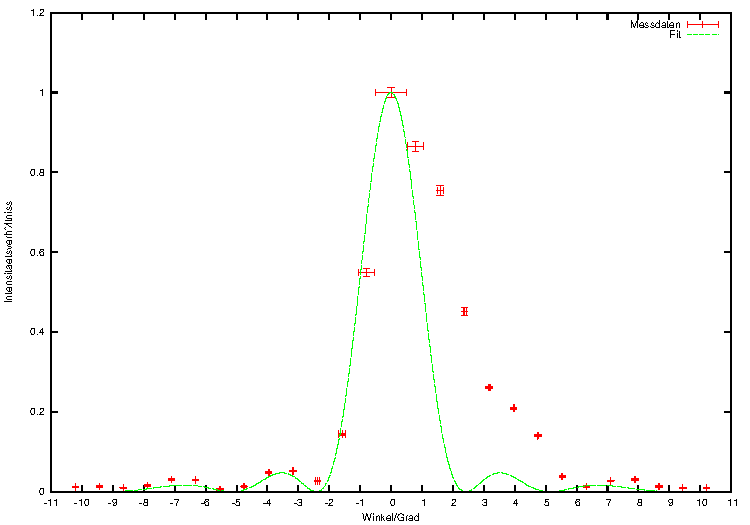
\includegraphics[scale = 1]{a_1.pdf}
  	\caption[Plot des Intensitätsverhältnisses in Abhängigkeit des Winkels, mit theoretischer Vorhersage]{Plot des Intensitätsverhältnisses in Abhängigkeit des Winkels, mit theoretischer Vorhersage}
  \label{fig:a_1}
\end{figure}

\subsection{Diskussion}
Die bestimmte Wellenlänge liegt im $\sigma_2$ Intervall des erwarteten Wertes von 0,63$\mu$m. Die Abweichung kann daher kommen, das der Spalt nicht exakt Parallel zur Messapparatur eingestellt war.
Die Messwerte liegen auf der linken Seite nah an der Theoriekurve, die Werte auf der rechten Seite Weichen stark ab. Die Abweichung zeigt sich auch in späteren Versuchsteilen. Es ist anzunehmen, dass die Lochblende des Laser auf der rechten Seite beschädigt ist, wodurch die Strahlen eine Streuung zur rechten Seite aufweisen und dort eine stärkere Intensität zu messen ist.


\section{Versuch WO3.2: Beugungsmuster einer Kreisblende}
\subsection{Versuchsdurchführung}

\subsubsection{Praktische Durchführung}
Wir verwenden den gleichen Aufbau wie bei Versuch WO3.1. Für diesen Versuch bestimmen wir aus dem Durchmesser der Kreislinie des ersten Minimums den Durchmesser der Lochblende und vergleichen unser Ergebnis mit dem auf der Lochblende angegebenen Wert. Wir bestimmen danch die Winkeldivergenz des Lichtbündels unseres Lasers.
\subsubsection{Theoretische Durchführung}
Der Durchmesser $D$ der Lochblende ist:
\begin{align}
D = \frac{3,8317 \lambda}{\sin(\theta)\pi}
\label{eqn:D}
\end{align}
$\lambda$ ist die Wellenlänge und $\theta$ der Winkel bis zum ersten Minimum. Der Vorfaktor 3,8317 kommt aus der Besselfunktion $I_1$.\\
Der zugehörige Fehler ist:
\begin{align}
\sigma_D = \sqrt{
\left(\frac{3,8317}{\sin(\theta)\pi}\sigma_\lambda \right)^2+
\left(\frac{3,8317\lambda}{\sin^2(\theta)\pi}\cos(\theta)
\sigma_\theta \right)^2}
\label{eqn:D_sigma}
\end{align}


\subsection{Messergebnisse}

\begin{table}[htbp]
\caption{Materialeigenschaften bei der Lochblende}
\begin{center}
\begin{tabular}{|l|l|l|l|l|l|}
\hline
Offset/mV & Fehler/mV & Durchmesser/mm & Fehler/mm & Abstand/m & Fehler/m \\ \hline
\multicolumn{1}{|r|}{-1,3} &  & \multicolumn{1}{r|}{0,25} & \multicolumn{1}{r|}{0,05} & \multicolumn{1}{r|}{1260} & \multicolumn{1}{r|}{0,02} \\ \hline
\end{tabular}
\end{center}
\label{tab:a_2_e}
\end{table}

\begin{table}[htbp]
\caption{Messwerte, der Vermessung der Lochblende}
\begin{center}
\begin{tabular}{|r|r|r|r|}
\hline
\multicolumn{1}{|l|}{Auslenkung/Grad} & \multicolumn{1}{l|}{Fehler/Grad} & \multicolumn{1}{l|}{Intensitätsverhältniss} & \multicolumn{1}{l|}{Fehler} \\ \hline
-0,59 & 0,02 & 0,003 & 0,001 \\ \hline
-0,55 & 0,02 & 0,003 & 0,001 \\ \hline
-0,50 & 0,02 & 0,003 & 0,001 \\ \hline
-0,45 & 0,02 & 0,003 & 0,001 \\ \hline
-0,41 & 0,02 & 0,003 & 0,001 \\ \hline
-0,36 & 0,02 & 0,022 & 0,001 \\ \hline
-0,32 & 0,02 & 0,042 & 0,001 \\ \hline
-0,27 & 0,02 & 0,032 & 0,001 \\ \hline
-0,23 & 0,02 & 0,032 & 0,001 \\ \hline
-0,18 & 0,02 & 0,013 & 0,001 \\ \hline
-0,14 & 0,02 & 0,109 & 0,001 \\ \hline
-0,09 & 0,02 & 0,380 & 0,002 \\ \hline
-0,045 & 0,02 & 0,768 & 0,006 \\ \hline
0 & 0,02 & 1 & 0,007 \\ \hline
0,045 & 0,02 & 0,932 & 0,007 \\ \hline
0,09 & 0,02 & 0,642 & 0,006 \\ \hline
0,14 & 0,02 & 0,245 & 0,005 \\ \hline
0,18 & 0,02 & 0,051 & 0,001 \\ \hline
0,23 & 0,02 & 0,013 & 0,001 \\ \hline
0,27 & 0,02 & 0,032 & 0,001 \\ \hline
0,32 & 0,02 & 0,013 & 0,001 \\ \hline
0,36 & 0,02 & -0,007 & 0,001 \\ \hline
0,41 & 0,02 & 0,003 & 0,001 \\ \hline
0,45 & 0,02 & 0,013 & 0,001 \\ \hline
0,50 & 0,02 & 0,0126 & 0,001 \\ \hline
0,55 & 0,02 & 0,003 & 0,001 \\ \hline
0,59 & 0,02 & -0,007 & 0,001 \\ \hline
\end{tabular}
\end{center}
\label{tab:a_2_m}
\end{table}



\subsection{Auswertung}
Es sollte der Durchmesser der Lochblende bestimmt werden, dafür wurde der Abstand zwischen den ersten beiden Minima verwendet und halbiert. Zur Berechnung des Durchmessers wurde Gleichung \ref{eqn:D} und Gleichung \ref{eqn:D_sigma} für den Fehler verwendet. Dabei ergab sich ein Wert von 0,30 $(\pm 0,05)$mm. Graphisch dargestellt ergibt sich die normierte Intensitätsverteilung (Werte aus Tabelle \ref{tab:a_2_m}).

\begin{figure}[H]
\centering
    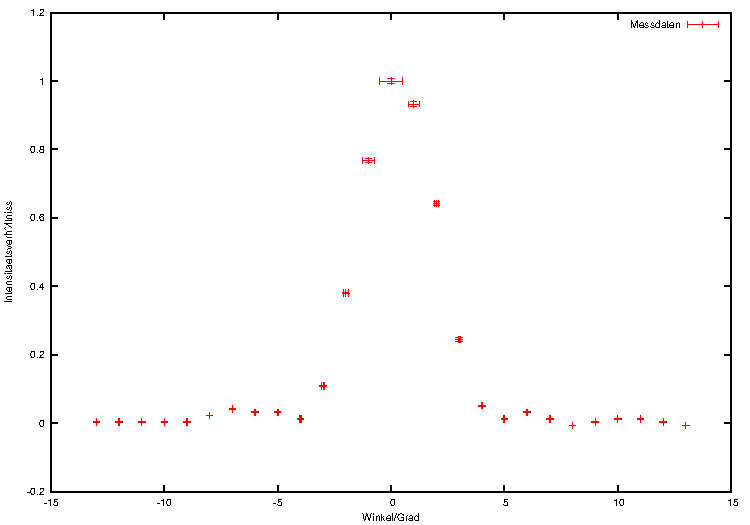
\includegraphics[scale = 1]{a_2.pdf}
  	\caption[Plot des Intensitätsverhältnisses in Abhängigkeit des Winkels, mit theoretischer Vorhersage]{Plot des Intensitätsverhältnisses in Abhängigkeit des Winkels, mit smooth csplines}
  \label{fig:a_2}
\end{figure}

\subsection{Diskussion}
Auf der Lochblende war ein Durchmesser von 0,2 mm angegeben, dieser Wert liegt erst im $\sigma_3$ Intervall des gemessenen Wertes. Diese Abweichung kann zum einen daher kommen, dass die Photozelle eine leichte Schrägstellung hat und zum anderen durch den defekt der Lochblende des Lasers, welcher auch in dieser Messung zu beobachten war.


\section{Versuch WO3.3: Beugungsmuster eines Doppelspaltes}
\subsection{Versuchsdurchführung}

\subsubsection{Praktische Durchführung}
Wir messen die Intensität des Doppelspaltes aus und stellen unsere Messergebnisse graphisch dar, sowie vergleichen sie mit der theoretischen Vorhersage. Wir berechnen danach die Wellenlänge.
\subsubsection{Theoretische Durchführung}
Die Wellenlänge $\lambda$ berechnet sich durch:
\begin{align}
\lambda = \frac{2d \sin(\theta)}{2n-1}
\label{eqn:lambda_2}
\end{align}
$n$ ist die Ordung des Minimums, d der Abstand des Doppelspaltes.
Der Fehler ergibt sich durch:
\begin{align}
\sigma_\lambda = \sqrt{
\left(\frac{2 \sin(\theta)}{2n-1}\sigma_d\right)^2+
\left(\frac{2d \cos(\theta)}{2n-1}\sigma_\theta\right)^2}
\label{eqn:lambda_2_sigma}
\end{align}
Für die Intensitätsverteilung $I_\theta$ erwarten wir folgenden Zusammenhang:
\begin{align}
I_\theta = I_0\left(\frac{\sin\left(\frac{\pi b \sin(\theta)}{\lambda}\right)}{\frac{\pi b \sin(\theta)}{\lambda}}\cos\left(\frac{\pi d\sin(\theta)}{\lambda}\right)\right)^2
\end{align}
$b$ ist dabei die Breite der Spalte, $d$ der Abstand der beiden Spalte und $\lambda$ die Wellenlänge des Lasers.

\subsection{Messergebnisse}

\begin{table}[htbp]
\caption{Materialeingenschaften, für die Messung des Doppelspaltes}
\begin{center}
\begin{tabular}{|l|l|l|l|}
\hline
Offset/mV & Fehler/mV & Durchmesser/mm & Fehler/mm \\ \hline
\multicolumn{1}{|r|}{-1,3} &  & \multicolumn{1}{r|}{0,25} & \multicolumn{1}{r|}{0,05} \\ \hline
Abstand schlitze/mm & Fehler/mm & Abstand/m & Fehler/m \\ \hline
\multicolumn{1}{|r|}{0,75} & \multicolumn{1}{r|}{0,05} & \multicolumn{1}{r|}{1260} & \multicolumn{1}{r|}{0,02} \\ \hline
\end{tabular}
\end{center}
\label{tab:a_3_e}
\end{table}



\begin{table}[htbp]
\caption{Messwerte, der Vermessung des Doppelspaltes}
\begin{center}
\begin{tabular}{|r|r|r|r|}
\hline
\multicolumn{1}{|l|}{Auslenkung/Grad} & \multicolumn{1}{l|}{Fehler} & \multicolumn{1}{l|}{Intensitätsverhältniss} & \multicolumn{1}{l|}{Fehler/Grad} \\ \hline
-0,8639 & 0,0001 & 0,0113762207 & 0,02 \\ \hline
-0,8184 & 0,0001 & 0,0023155139 & 0,02 \\ \hline
-0,7729 & 0,0001 & 0,0053357495 & 0,02 \\ \hline
-0,7275 & 0,0001 & 0,0174166918 & 0,02 \\ \hline
-0,6820 & 0,0001 & 0,0023155139 & 0,02 \\ \hline
-0,6365 & 0,0001 & 0,0103694755 & 0,01 \\ \hline
-0,5911 & 0,0001 & 0,0244639082 & 0,02 \\ \hline
-0,5456 & 0,0001 & 0,0023155139 & 0,02 \\ \hline
-0,5001 & 0,0001 & 0,0194301822 & 0,02 \\ \hline
-0,4547 & 0,0001 & 0,0405718313 & 0,02 \\ \hline
-0,4092 & 0,0001 & 0,0023155139 & 0,02 \\ \hline
-0,3637 & 0,0001 & 0,0435920668 & 0,02 \\ \hline
-0,3183 & 0,0001 & 0,0848686198 & 0,02 \\ \hline
-0,2728 & 0,0001 & 0,0033222591 & 0,02 \\ \hline
-0,2273 & 0,0001 & 0,1311788986 & 0,02 \\ \hline
-0,1819 & 0,0002 & 0,242927615 & 0,02 \\ \hline
-0,1364 & 0,0001 & 0,0113762207 & 0,02 \\ \hline
-0,0909 & 0,0007 & 0,9073794423 & 0,02 \\ \hline
-0,0454 & 0,0007 & 1 & 0,01 \\ \hline
0 & 0,0007 & 1 & 0,02 \\ \hline
0,0454 & 0,0007 & 1 & 0,02 \\ \hline
0,0909 & 0,0005 & 1 & 0,01 \\ \hline
0,1364 & 0,0001 & 0,0214436726 & 0,02 \\ \hline
0,1819 & 0,0001 & 0,1563475284 & 0,02 \\ \hline
0,2273 & 0,0001 & 0,1221181919 & 0,02 \\ \hline
0,2728 & 0,0001 & 0,0043290043 & 0,02 \\ \hline
0,3183 & 0,0001 & 0,0647337159 & 0,02 \\ \hline
0,3637 & 0,0001 & 0,0375515957 & 0,02 \\ \hline
0,4092 & 0,0001 & 0,0023155139 & 0,02 \\ \hline
0,4547 & 0,0001 & 0,0315111245 & 0,02 \\ \hline
0,5002 & 0,0001 & 0,0164099466 & 0,02 \\ \hline
0,5456 & 0,0001 & 0,0013087688 & 0,02 \\ \hline
0,5911 & 0,0001 & 0,0194301822 & 0,02 \\ \hline
0,6366 & 0,0001 & 0,0103694755 & 0,02 \\ \hline
0,6820 & 0,0001 & 0,0023155139 & 0,02 \\ \hline
0,7275 & 0,0001 & 0,0133897111 & 0,02 \\ \hline
0,7729 & 0,0001 & 0,0053357495 & 0,02 \\ \hline
0,8185 & 0,0001 & 0,0013087688 & 0,02 \\ \hline
0,8639 & 0,0001 & 0,0073492399 & 0,02 \\ \hline
0,9094 & 0,0001 & 0,0023155139 & 0,02 \\ \hline
0,9548 & 0,0001 & 0,0013087688 & 0,02 \\ \hline
\end{tabular}
\end{center}
\label{tab:a_3_m}
\end{table}


\subsection{Auswertung}
In der dritten Aufgabe sollte der Intensitätsverlauf eines Doppelspaltes gemessen werden und nach Gleichung \ref{eqn:lambda_2} und Gleichung \ref{eqn:lambda_2_sigma} für den Fehler die Wellenlänge des Lasers bestimmt werden. Es ergab sich ein Werte von 0,069 $(\pm 0,008) \mu$m.
Graphisch ausgewertet ergibt sich der folgende Plot (Werte aus Tabelle \ref{tab:a_3_m}).

\begin{figure}[H]
\centering
    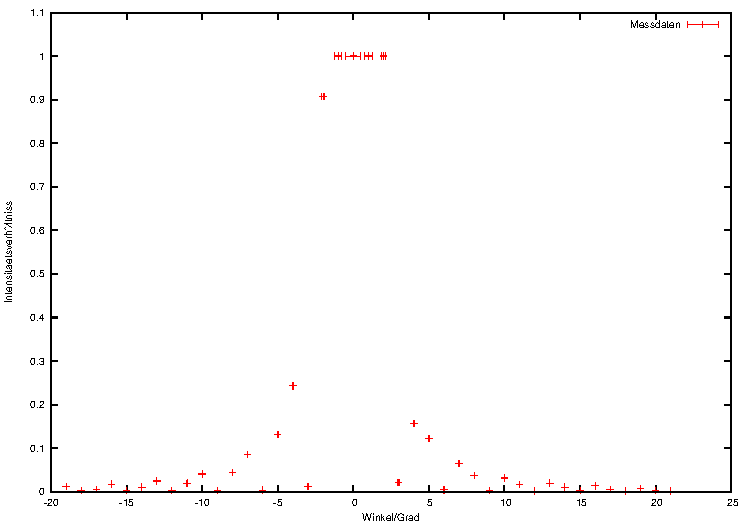
\includegraphics[scale = 1]{a_3.pdf}
  	\caption[Plot des Intensitätsverhältnisses in Abhängigkeit des Winkels, mit theoretischer Vorhersage]{Plot des Intensitätsverhältnisses in Abhängigkeit des Winkels, mit theoretischer Vorhersage}
  \label{fig:a_1}
\end{figure}


\subsection{Diskussion}
Der erwartete Wert für die Wellenlänge war 0,63$\mu$m, dieser liegt innerhalb des $\sigma_1$ Intervalls, des gemessenen Wertes 0,069 $(\pm 0,008) \mu$m. Die Theoretische Vorhersage weicht stark vom den gemessenen Werten ab, dies betrifft jedoch nur die Amplitude, nicht die Position der Minima und Maxima. Der Fehler kommt daher, dass das Messgerät eine Begrenzung von 992 mV hat, dieser Umstand uns jedoch nicht bekannt war. Dieser Fehler hätte mit einem Intensitätsfilter behoben werden können.

\section{Versuch WO3.4: Beugungsmuster eines Gitters}
\subsection{Versuchsdurchführung}

\subsubsection{Praktische Durchführung}
Bei dem in diesem Versuchsteil verwendeten Gitter liegt die Gitterkonstante im Bereich von ca. 10$^{-2}$cm. Wir bestimmen aus der Intensitätsverteilung und der Gitterkonstante $d$ die Wellenlänge des Laserlichtes.
\subsubsection{Theoretische Durchführung}
Die Wellenlänge $\lambda$ bestimmen wir durch die Formel:
\begin{align}
\lambda = \frac{\sin(\theta) d}{n}
\end{align}
$d$ ist die Gitterkonstante, $n$ die Ordnung des Maximums und $\theta$ die Winkeldifferenz zwischen Hauptmaximum und Nebenmaximum.
Der Fehler berechnet sich durch:
\begin{align}
\sigma_\lambda = \sqrt{
\left(\frac{\cos(\theta) d}{n}\sigma_\theta\right)^2+
\left(\frac{\sin(\theta)}{n}\sigma_d\right)^2}
\end{align}
Für die Intensitätsverteilung $I_\theta$ erwarten wir folgenden Zusammenhang:
\begin{align}
I_\theta = I_0\left(\frac{\sin\left(\frac{\pi d \sin(\theta)}{2\lambda}\right)}{\frac{\pi d \sin(\theta)}{2\lambda}}
\frac{\sin\left(\frac{N \pi d \sin(\theta)}{\lambda}\right)}{\sin\left(\frac{\pi d \sin(\theta)}{\lambda}\right)}\right)^2
\end{align}
$b$ ist dabei die Breite der Spalte, $d$ der Abstand der beiden Spalte und $\lambda$ die Wellenlänge des Lasers.

\subsection{Messergebnisse}
\subsection{Auswertung}
\subsection{Diskussion}
\subsection{Messergebnisse}



\section{Fazit}


 %Werte stimmen mit den Formeln überein/nicht überein

\end{document}

